\typeout{(body.tex)}

\begin{frame}
    \titlepage
\end{frame}

% Introduction:
    % do we need more than lists?
        % better than linear search
        % complex relationships
            % examples: language tree, phylogenic
    % relationships between nodes
        % list as up to 2
        % binary tree as up to 3
\begin{frame}{are lists enough?}
\begin{itemize}
    \item for correctness --- sure
    \vspace{.5cm}
    \item want to efficiently access items
        \begin{itemize}
        \item \myemph{better than linear time} to find something
        \end{itemize}
    \item want to \myemph{represent relationships} more naturally
\end{itemize}
\end{frame}

\begin{frame}{inter-item relationships in lists}
\begin{tikzpicture}
\tikzset{>=Latex}
\node[draw] (n1) { 1 };
\node[draw,right=1cm of n1] (n2) { 2 };
\node[draw,right=1cm of n2] (n3) { 3 };
\node[draw,right=1cm of n3] (n4) { 4 };
\node[draw,right=1cm of n4] (n5) { 5 };
\foreach \x/\y in {1/2,2/3,3/4,4/5} {
    \draw[ultra thick,<->] (n\x) -- (n\y);
}
\end{tikzpicture}
\begin{itemize}
\item List: \textit{nodes} related to \myemph{predecessor}/\myemph{successor}
\end{itemize}
\end{frame}

\begin{frame}{trees}
\begin{itemize}
    \item trees: allow representing more relationships
        \begin{itemize}
        \item (but not arbitrary relationships --- see graphs later in semester)
        \end{itemize}
    \item restriction: single path from \textit{root} to every node
        \begin{itemize}
        \item implies single path from every node to every other node (possibly through root)
        \end{itemize}
\end{itemize}
\end{frame}

\begin{frame}{natural trees: phylogenetic tree}
\vspace{-.25cm}
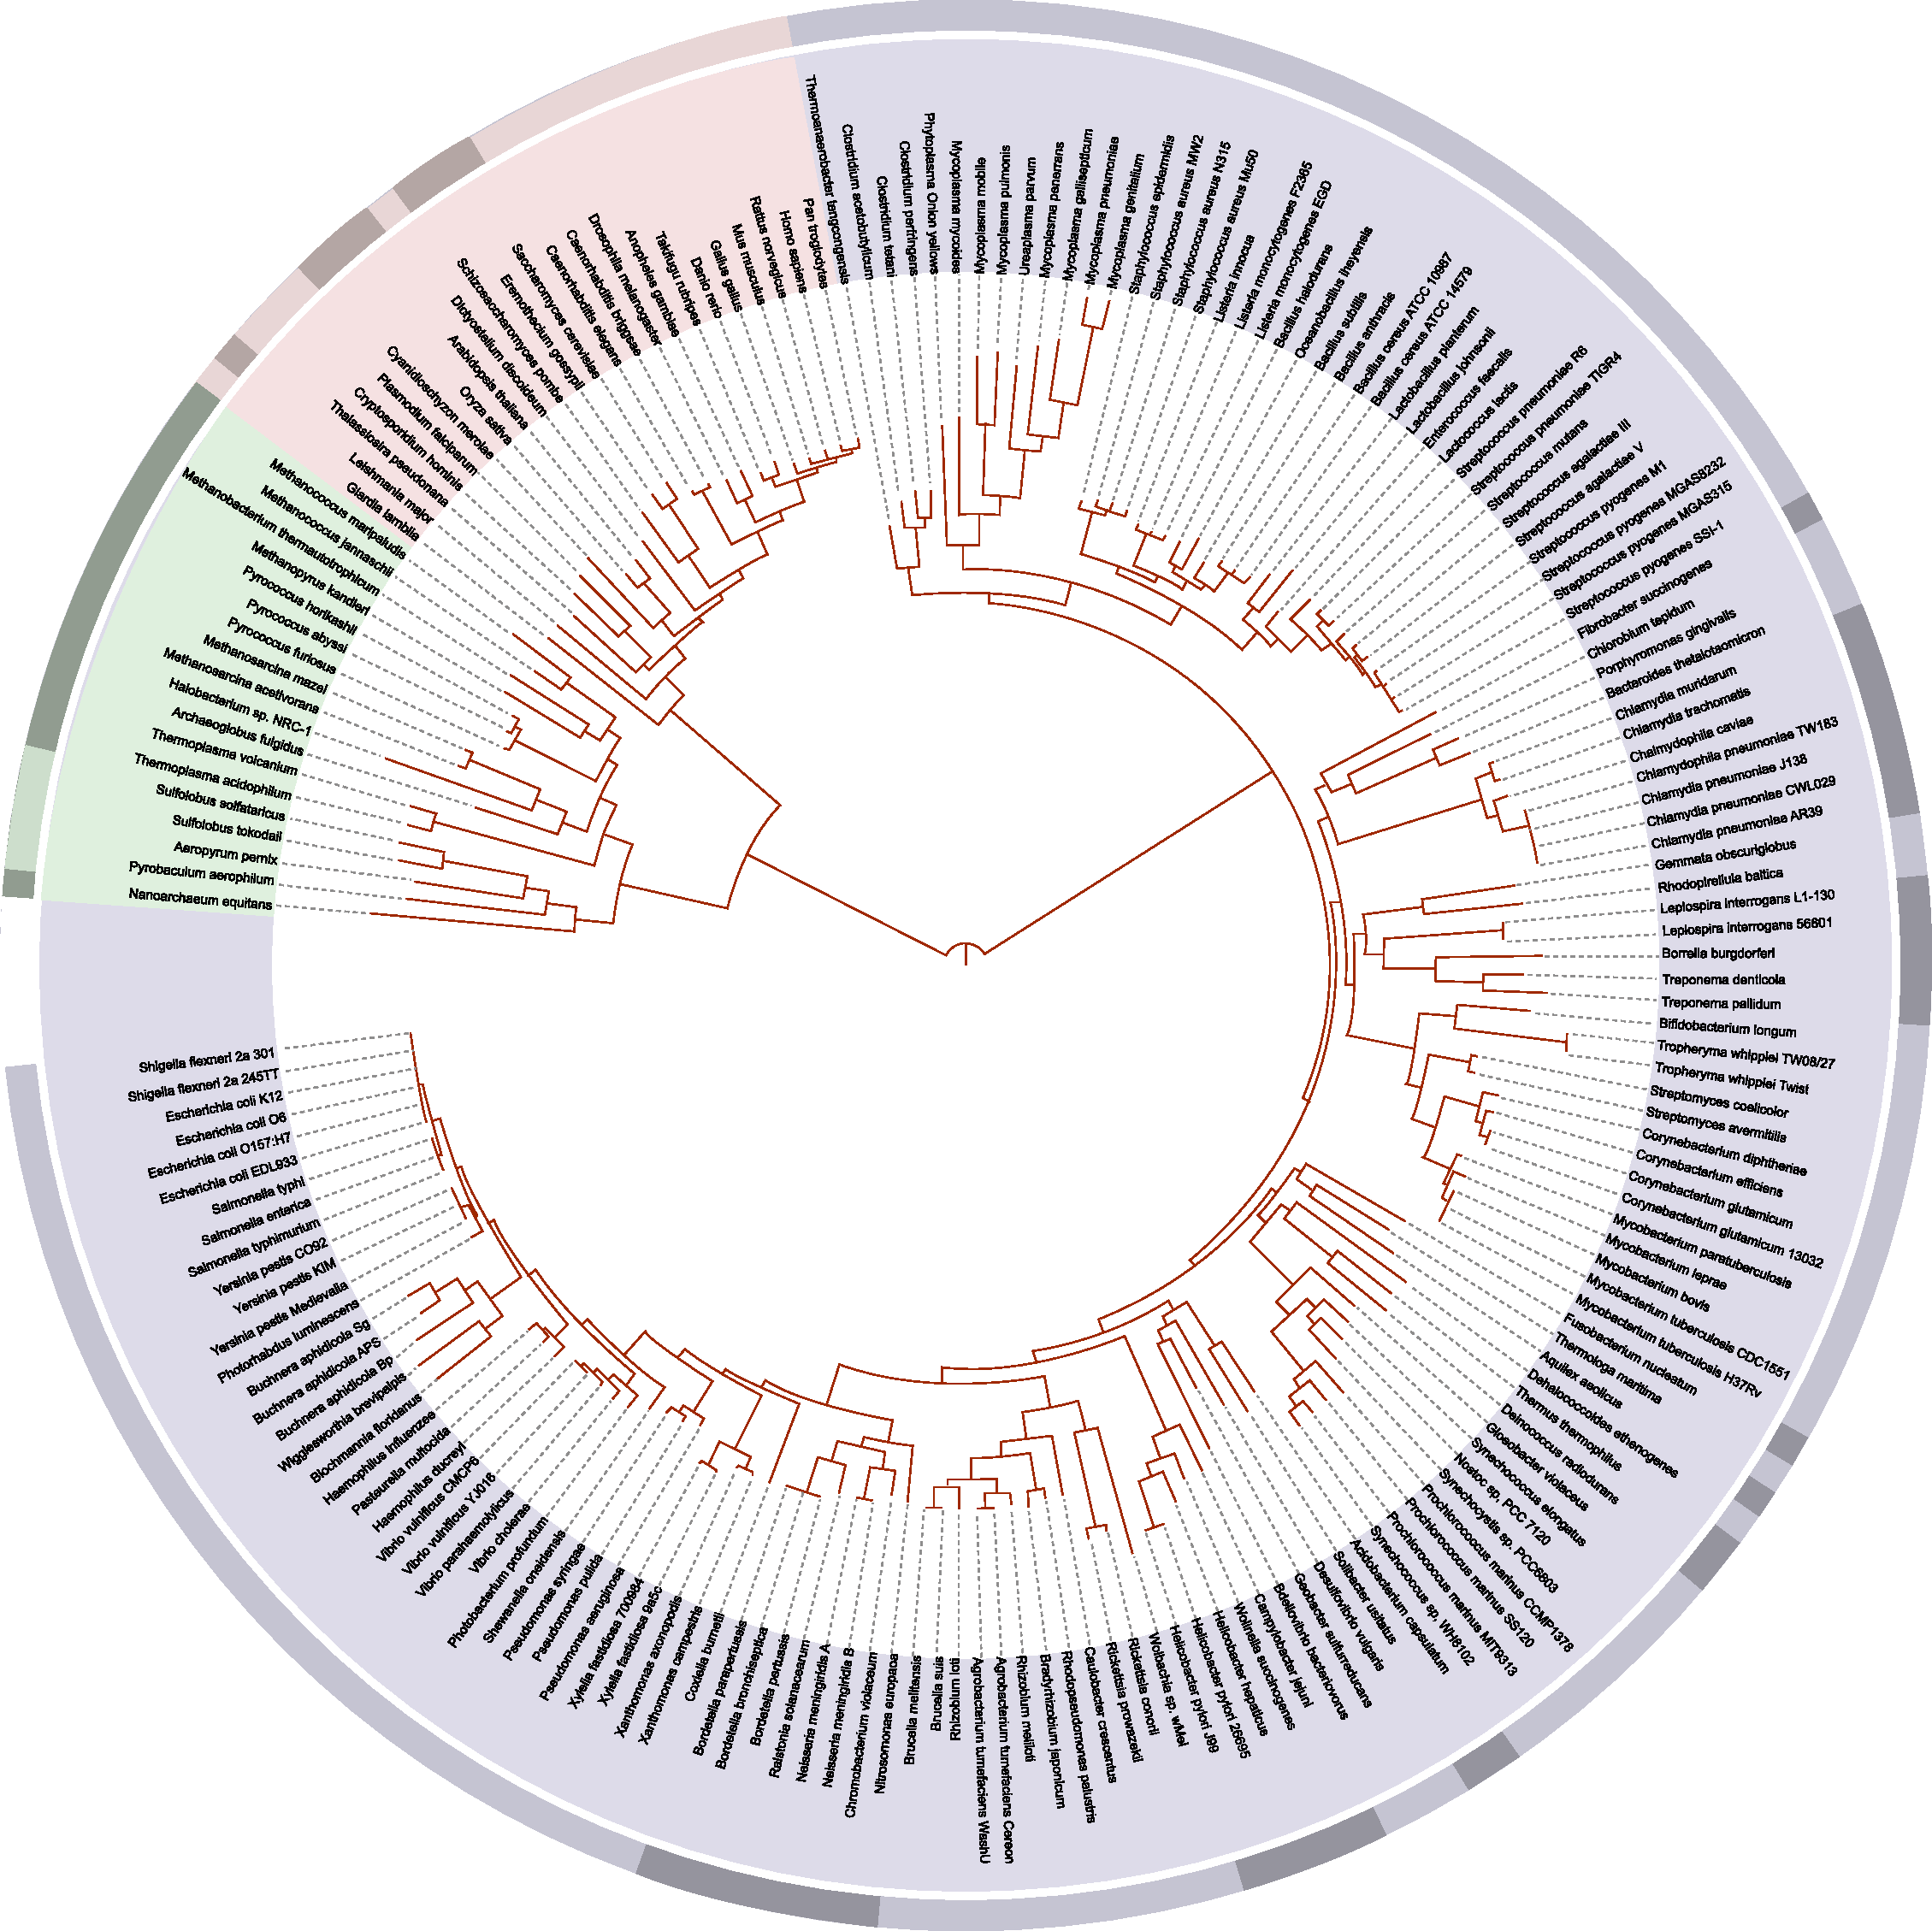
\includegraphics[height=0.9\textheight]{Tree_of_Life}
\imagecredit{image: Ivicia Letunic and Mariana Ruiz Villarreal, via the tool iTOL (Interative Tree of Life), via Wikipedia}
\end{frame}

\begin{frame}{natural trees: phylogenetic tree (zoom)}
\vspace{-.25cm}
    \adjincludegraphics[height=0.9\textheight,trim={{0\width} {0\height} {.25\height} {.6\width}},clip]{Tree_of_Life}
\imagecredit{image: Ivicia Letunic and Mariana Ruiz Villarreal, via the tool iTOL (Interative Tree of Life), via Wikipedia}
\end{frame}

\begin{frame}{natural trees: Indo-European languages}
\vspace{-.25cm}
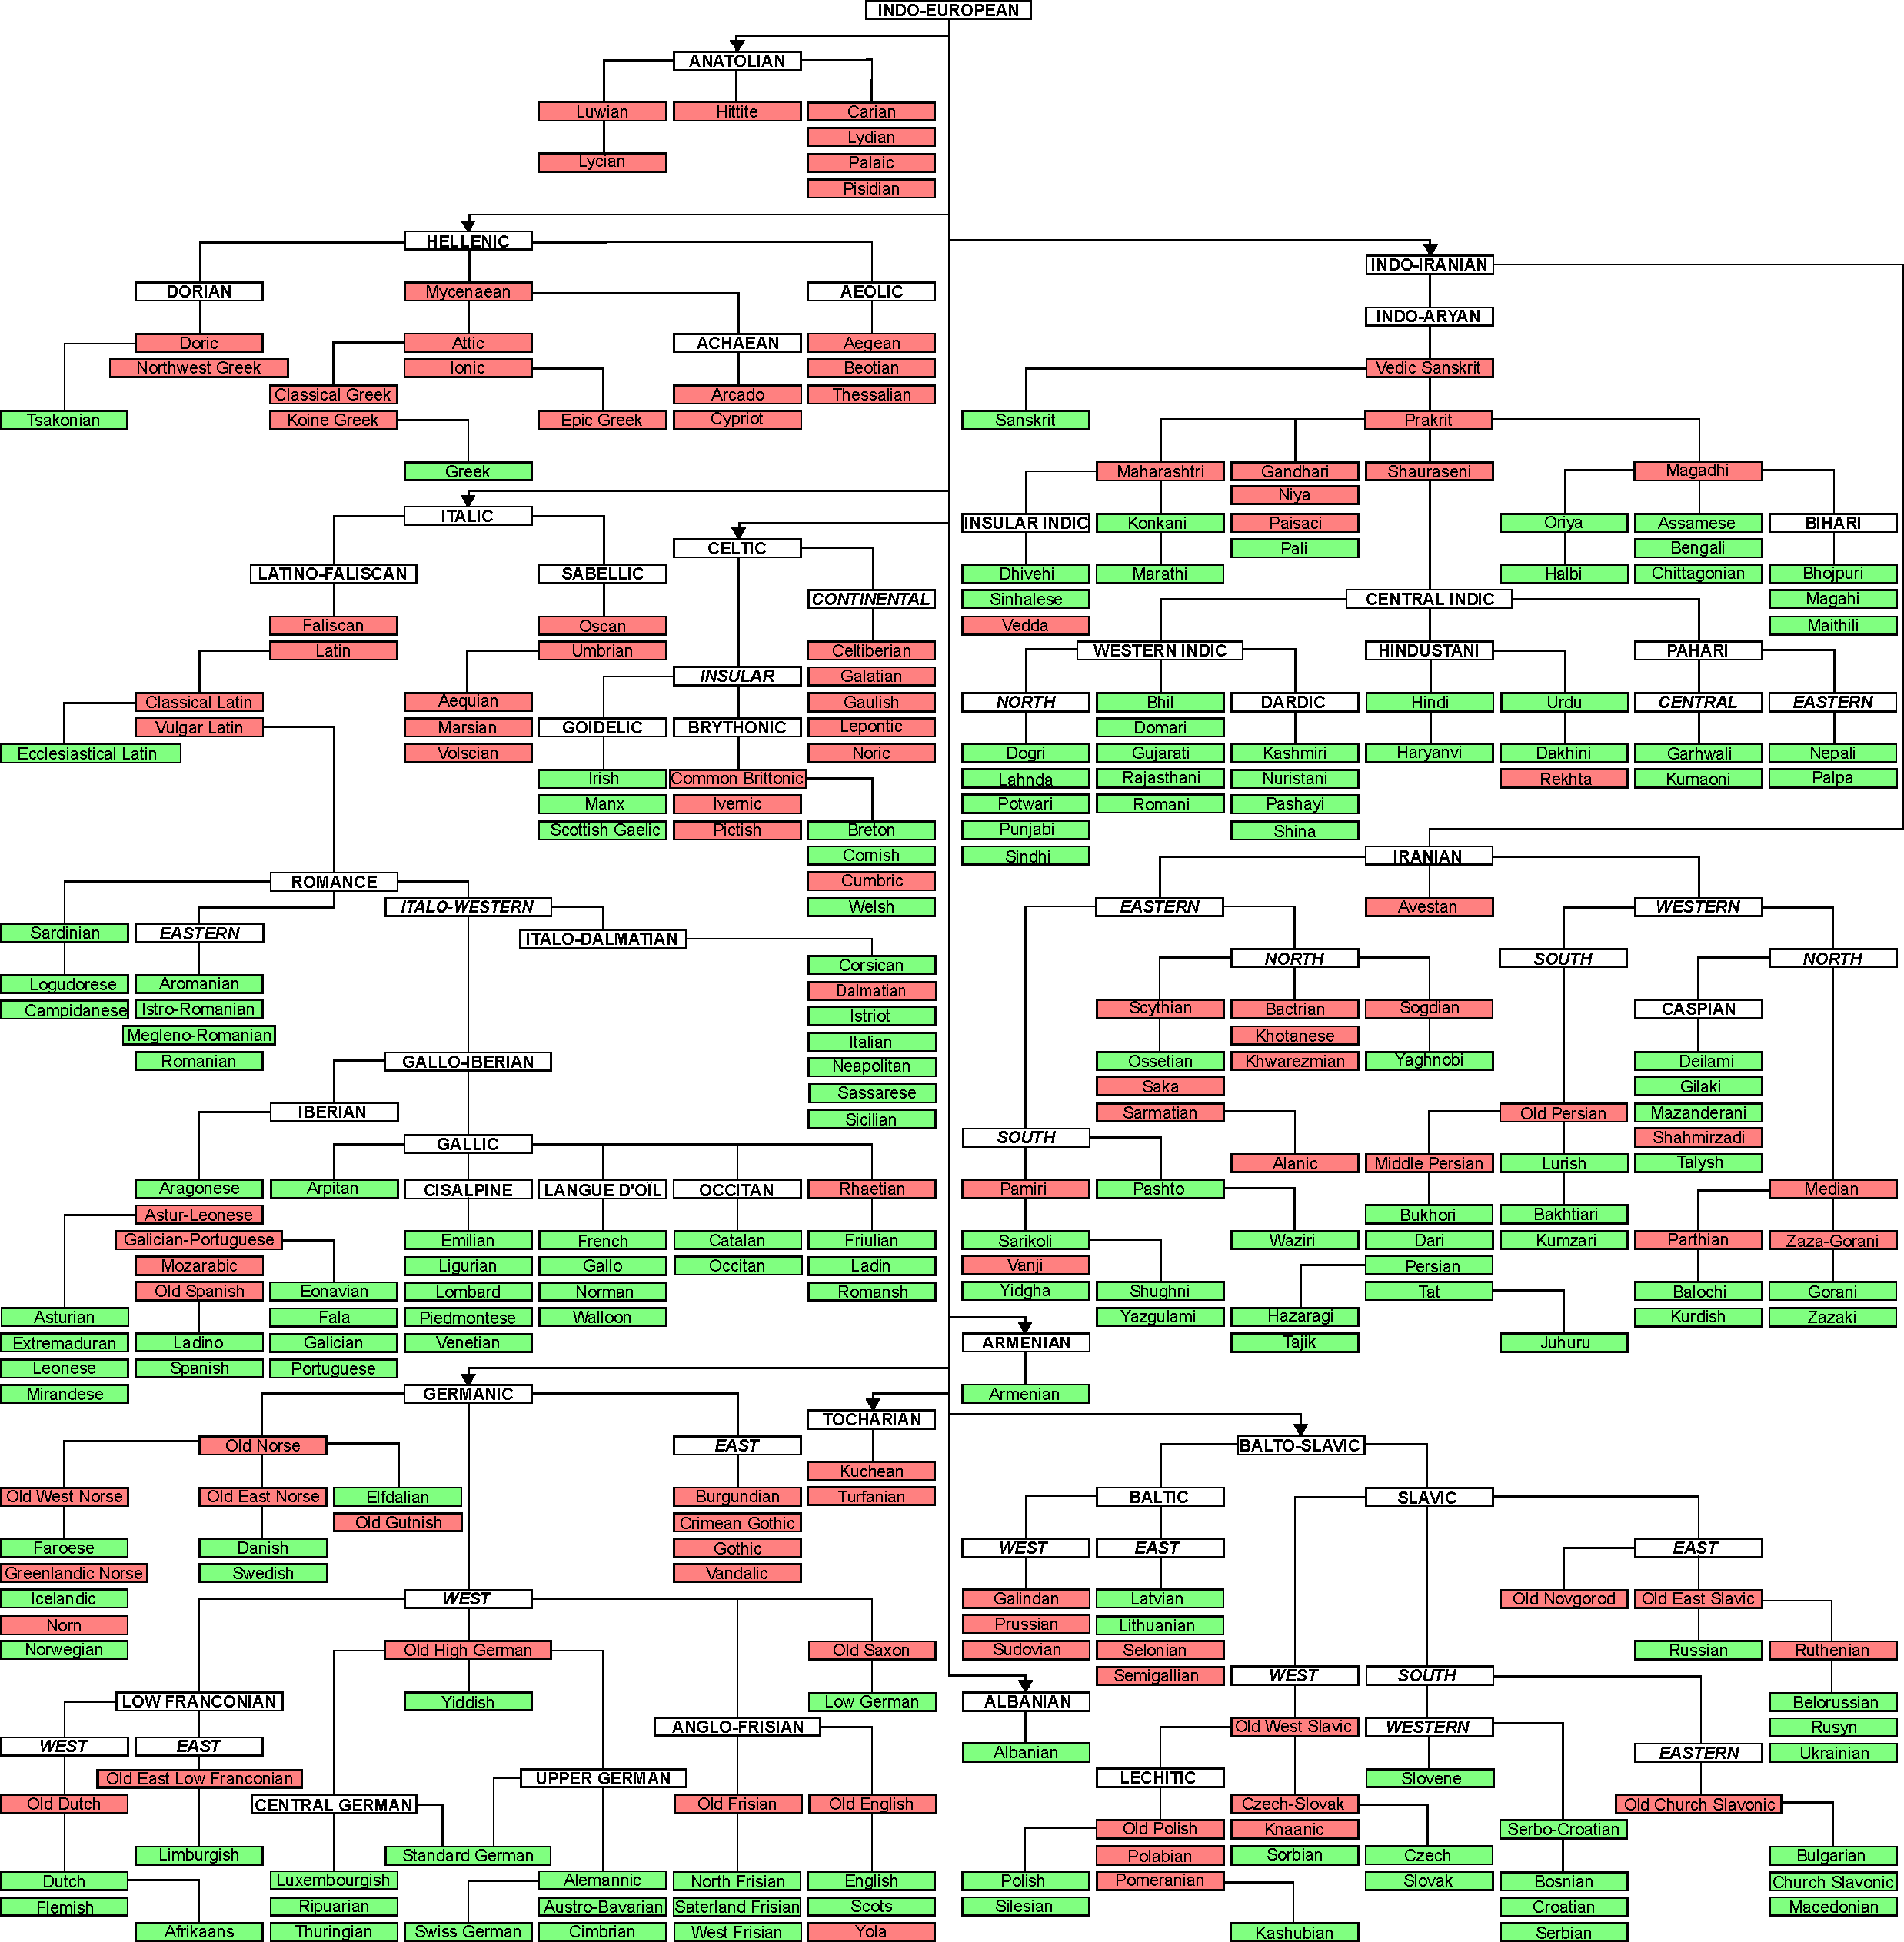
\includegraphics[height=0.9\textheight]{IndoEuropeanTree}
\imagecredit{image: via Wikipedia/Mandrak}
\end{frame}

\begin{frame}{list to tree}
\begin{tikzpicture}
\tikzset{>=Latex}
\begin{scope}[start chain=going right,every join/.style={->,very thick}]
\node[draw,thick,on chain] {predecessor};
\node[draw,thick,on chain,join] (elem) {element};
\node[draw,thick,on chain,join] {successor};
\end{scope}
\node[above=.5cm of elem] {\textit{list} --- up to 2 related nodes};

\node[draw,below=2cm of elem] (parent) {parent};
\node[draw,below=1cm of parent] (elem2) {element};
\node[draw,below=1cm of elem2,xshift=-2cm] (leftChild) {left child};
\node[draw,below=1cm of elem2,xshift=2cm] (rightChild) {left child};
\draw[->,very thick] (parent) -- (elem2);
\draw[->,very thick] (elem2) -- (leftChild);
\draw[->,very thick] (elem2) -- (rightChild);
\node[above=.5cm of parent] {\textit{binary tree} --- up to 3 related nodes (list is special-case)};
\end{tikzpicture}
\end{frame}

\begin{frame}{more general trees}
\begin{tikzpicture}
\tikzset{>=Latex}
\node[draw] (parent) {parent};
\node[draw,below=1cm of parent] (elem2) {element};
\node[draw,below=1cm of elem2,xshift=-4cm] (leftChild) {child 1};
\node[draw,below=1cm of elem2,xshift=0cm] (middleChild) {child 2};
\node[draw,below=1cm of elem2,xshift=5cm] (rightChild) {child $n$};
\node[font=\large,left=1.5cm of rightChild]{\ldots};
\draw[->,very thick] (parent) -- (elem2);
\draw[->,very thick] (elem2) -- (leftChild);
\draw[->,very thick] (elem2) -- (middleChild);
\draw[->,very thick] (elem2) -- (rightChild);
\node[above=.5cm of parent,align=left] {\textit{tree} --- any number of relationships (binary tree is special case) \\ \hspace{2cm}at most one parent};
\end{tikzpicture}
\end{frame}


    % tree vocab
        % root/leaf/sibling/height (of node, of tree)/depth of node
        % path/length of path/*internal path length
\begin{frame}[fragile,label=treeTerms1]{tree terms (1)}
\newcommand{\term}[1]{\textit{\textbf{#1}}}
\begin{tikzpicture}
\tikzset{
    >=Latex,
    treeNode/.style={draw, thick},
    treeConnect/.style={draw, very thick,->},
    nameLabel/.style={ultra thick,<-},
}
\tikzset{
    leafColor/.style={blue!70!black},
    siblingColor/.style={green!70!black},
}
\node[treeNode] (a) {A};
\node[treeNode,below=1cm of a,xshift=-1cm] (b) {B};
\node[treeNode,below=1cm of a,xshift=1cm] (c) {C};
\node[treeNode,below=1cm of c,xshift=-.5cm] (e) {E};
\node[treeNode,below=1cm of c,xshift=1cm] (f) {F};
\node[treeNode,below=1cm of c,xshift=3cm] (g) {G};
\node[treeNode,below=1cm of b,xshift=-.5cm] (d) {D};
\node[treeNode,below=1cm of d] (h) {H};

\foreach \x/\y in {a/b,a/c,c/e,c/f,c/g,b/d,d/h} {
    \draw[treeConnect] (\x) -- (\y);
}

\node at ([xshift=2cm,yshift=.5cm]a.north) (parentKey) { parent };
\draw[treeConnect] (parentKey.east) -- ++(1cm,0cm) node[right] { child };
\draw[nameLabel,orange!70!black] ([xshift=.5mm]a.east) -- ++(2cm,0cm) node[right] { \term{root}: node with no parents };
\draw[nameLabel,leafColor] ([yshift=-.5mm]g.south) -- ++(-1cm,-1cm) node[right] (leafsLabel) { \term{leafs}: nodes with no children };
\draw[nameLabel,leafColor] ([yshift=-.5mm]f.south) -- (leafsLabel.west);
\draw[nameLabel,leafColor] ([yshift=-.5mm]e.south) -- (leafsLabel.west);
\draw[nameLabel,leafColor] ([xshift=.5mm]h.east) -- (leafsLabel.west);

\node[draw,fill=green!70!black,fill opacity=0.025,inner sep=0mm,ellipse,nameLabel,siblingColor,fit=(e) (f) (g)] (siblingEllip) {};
\node[above right=.1mm of siblingEllip,siblingColor] { \term{siblings}: nodes with the same parent};
\end{tikzpicture}
\end{frame}

\begin{frame}[fragile,label=paths]{paths and path lengths}
\newcommand{\term}[1]{\textit{\textbf{#1}}}
\begin{tikzpicture}
\tikzset{
    >=Latex,
    treeNode/.style={draw, thick},
    treeConnect/.style={draw, very thick,->},
    nameLabel/.style={ultra thick,<-},
}
\tikzset{
    pathColor/.style={orange!70!black}
}
\node[treeNode] (a) {A};
\node[pathColor,treeNode,below=1cm of a,xshift=-1cm] (b) {B};
\node[treeNode,below=1cm of a,xshift=1cm] (c) {C};
\node[treeNode,below=1cm of c,xshift=-.5cm] (e) {E};
\node[treeNode,below=1cm of c,xshift=1cm] (f) {F};
\node[treeNode,below=1cm of c,xshift=3cm] (g) {G};
\node[pathColor,treeNode,below=1cm of b,xshift=-.5cm] (d) {D};
\node[pathColor,treeNode,below=1cm of d] (h) {H};

\foreach \x/\y in {a/b,a/c,c/e,c/f,c/g,b/d,d/h} {
    \draw[treeConnect] (\x) -- (\y);
}
\draw[treeConnect,orange] (b) -- (d);
\draw[treeConnect,orange] (d) -- (h);
    \coordinate (childKey) at ([xshift=1cm]parentKey.east);
\node[below right=.5cm and -3cm of childKey,pathColor,align=left] (pathDesc) { \term{path}: sequence of nodes $n_1, n_2, \ldots, n_k$ \\ \hspace{2cm} such that $n_i$ is parent of $n_{i+1}$  \\
example: $\{B, D, H\}$};
\node[align=left,anchor=north west] (lengthDesc) at ([yshift=-.5cm,xshift=-3cm]g.south west) { \term{length} (of path): number of \textit{edges} in path \\ example: 2 ($B\rightarrow D$ and $D\rightarrow H$) };

\node[align=left,anchor=north west] (iLengthDesc) at ([yshift=-.5cm]lengthDesc.south west) { \term{internal path length}: sum of depth of nodes \\ example: $6 = 1 + 2 + 3$ };
\end{tikzpicture}
\end{frame}

\begin{frame}[fragile,label=nodeHeight]{tree/node height}
\newcommand{\term}[1]{\textit{\textbf{#1}}}
\begin{tikzpicture}
\tikzset{
    >=Latex,
    treeNode/.style={draw, thick},
    treeConnect/.style={draw, very thick,->},
    nameLabel/.style={ultra thick,<-},
}
\tikzset{
    heightColor/.style={orange!70!black}
}
\node[treeNode] (a) {A};
\node[treeNode,below=1cm of a,xshift=-1cm] (b) {B};
\node[treeNode,below=1cm of a,xshift=1cm] (c) {C};
\node[treeNode,below=1cm of c,xshift=-.5cm] (e) {E};
\node[treeNode,below=1cm of c,xshift=1cm] (f) {F};
\node[treeNode,below=1cm of c,xshift=3cm] (g) {G};
\node[treeNode,below=1cm of b,xshift=-.5cm] (d) {D};
\node[treeNode,below=1cm of d] (h) {H};

\foreach \x/\y in {a/b,a/c,c/e,c/f,c/g,b/d,d/h} {
    \draw[treeConnect] (\x) -- (\y);
}

\node at ([xshift=2cm,yshift=.5cm]a.north) (parentKey) { parent };
\draw[treeConnect] (parentKey.east) -- ++(1cm,0cm) node[right] (childKey) { child };
\node[below right=.5cm and -3cm of childKey,heightColor] (heightDesc) { \term{height} (of a node): length of longest path to leaf };
\node[below=1cm of heightDesc,heightColor,align=left] (heightDesc2) { \term{height} (of a tree): height of tree's root \\ \hspace{2cm}(this example: 3) };
\node[heightColor,right=0cm of a] {3};
\node[heightColor,right=0cm of b] {2};
\node[heightColor,right=0cm of d] {1};
\node[heightColor,right=0cm of h] {0};
\node[heightColor,right=0cm of c] {1};
\node[heightColor,right=0cm of e] {0};
\node[heightColor,right=0cm of f] {0};
\node[heightColor,right=0cm of g] {0};
\end{tikzpicture}
\end{frame}

\begin{frame}[fragile,label=nodeDepth]{tree/node depth}
\newcommand{\term}[1]{\textit{\textbf{#1}}}
\begin{tikzpicture}
\tikzset{
    >=Latex,
    treeNode/.style={draw, thick},
    treeConnect/.style={draw, very thick,->},
    nameLabel/.style={ultra thick,<-},
}
\tikzset{
    depthColor/.style={green!70!black}
}
\node[treeNode] (a) {A};
\node[treeNode,below=1cm of a,xshift=-1cm] (b) {B};
\node[treeNode,below=1cm of a,xshift=1cm] (c) {C};
\node[treeNode,below=1cm of c,xshift=-.5cm] (e) {E};
\node[treeNode,below=1cm of c,xshift=1cm] (f) {F};
\node[treeNode,below=1cm of c,xshift=3cm] (g) {G};
\node[treeNode,below=1cm of b,xshift=-.5cm] (d) {D};
\node[treeNode,below=1cm of d] (h) {H};

\foreach \x/\y in {a/b,a/c,c/e,c/f,c/g,b/d,d/h} {
    \draw[treeConnect] (\x) -- (\y);
}

\node at ([xshift=2cm,yshift=.5cm]a.north) (parentKey) { parent };
\draw[treeConnect] (parentKey.east) -- ++(1cm,0cm) node[right] (childKey) { child };
\node[below right=.5cm and -3cm of childKey,depthColor] (depthDesc) { \term{depth} (of a node): length of path to root };
\node[depthColor,right=0cm of a] {0};
\node[depthColor,right=0cm of b] {1};
\node[depthColor,right=0cm of d] {2};
\node[depthColor,right=0cm of h] {3};
\node[depthColor,right=0cm of c] {1};
\node[depthColor,right=0cm of e] {2};
\node[depthColor,right=0cm of f] {2};
\node[depthColor,right=0cm of g] {2};
\end{tikzpicture}
\end{frame}



% FIXME: CHECK internal path length

    % ? example with language tree

% FIXME: tree examples
    % tree examples:
        % parse, genology, expression

\begin{frame}[fragile,label=firstChildNextSib]{first child/next sibling}
\lstset{
    language=C++,
    style=small
}
\begin{tikzpicture}
\node (code) {
\begin{lstlisting}
class TreeNode {
  private:
    string element;
    TreeNode *firstChild;
    TreeNode *nextSibling;
  public:
    ...
};
\end{lstlisting}
};
\begin{scope}[xscale=.5,yscale=.75]
\tikzset{
    g/.style={draw,thick,font=\small},
    c/.style={draw,-Latex,very thick},
}
\node[g] at ([xshift=3cm]code.north east) (home) {home};
\node[g,below=1cm of home] (aaron) {aaron}; \draw[c] (home) -- (aaron);
\node[g,below=1cm of aaron,draw=red!90!black] (cs2150) {cs2150}; \draw[c] (aaron) -- (cs2150);
\node[g,right=1.5cm of cs2150] (cs4970) {cs4970}; \draw[c,draw=red!90!black] (cs2150) -- (cs4970);
    \draw[red] ($(cs2150)!.5!(cs4970)$) -- ++(0cm,.5cm) node[red!90!black,above,inner sep=0.5mm,font=\small\tt] {nextSibling};
\node[g,right=1.5cm of cs4970] (mail) {mail}; \draw[c] (cs4970) -- (mail);
\node[g,below=1cm of cs2150] (lab1) {lab1}; \draw[c,draw=red!90!black] (cs2150) -- (lab1);
    \draw[red] ($(cs2150)!.5!(lab1)$) -- ++(-.5cm,0cm) node[red!90!black,left,inner sep=0.5mm,font=\small\tt] {firstChild};
\node[g,right=1.5cm of lab1] (lab2) {lab2}; \draw[c] (lab1) -- (lab2);
\node[g,right=1.5cm of lab2] (proj1) {proj1}; \draw[c] (lab2) -- (proj1);
\node[g,below=1cm of proj1] (projH) {proj.h}; \draw[c] (proj1) -- (projH);
\node[g,below=1cm of lab1] (collH) {coll.h}; \draw[c] (lab1) -- (collH);
\node[g,right=1.5cm of collH] (collCpp) {coll.cpp}; \draw[c] (collH) -- (collCpp);
\end{scope}
\end{tikzpicture}
\end{frame}

    % TreeNode: firstChild/nextSibling

\usetikzlibrary{graphs}
\usetikzlibrary{graphdrawing}
\usegdlibrary{trees}

\begin{frame}{tree traversal}
\begin{tikzpicture}
\graph[tree layout,
    nodes={draw,thick,circle,text width=.25cm,align=center,text height=.25cm,text depth=0cm},
    edges={thick,-Latex}] {
    [fresh nodes] 
        "$/$" -> {
            "$\times$" -> {
                "+" -> {
                    [name=plus] 1, 2
                },
                "-" -> {
                    [name=minus] 3, 4
                },
            },
            "$\times$" -> {
                [name=times] 5, 6
            }
        }
};
\node[anchor=north west,align=left]  at ([yshift=-1cm]plus 1.south west){
    pre-order: {\tt / * + 1 2 - 3 4 * 5 6} \\
    in-order: {\tt (((1+2) * (3-4)) / (5*6))} (parenthesis optional?) \\
    post-order: {\tt 1 2 + 3 4 - * 5 6 * / } \\
};
\end{tikzpicture}
\end{frame}

\begin{frame}[fragile,label=prePostPrint]{pre/post-order traversal printing}
\lstset{language=C++,style=small}
(this is pseudocode)
\begin{lstlisting}
TreeNode::printPreOrder() {
    this->print();
    for each child c of this:
        c->printPreOrder()
}

TreeNode::printPostOrder() {
    for each child c of this:
        c->printPostOrder()
    this->print();
}
\end{lstlisting}
\end{frame}

\begin{frame}[fragile,label=inPrint]{in-order traversal printing}
\lstset{language=C++,style=small}
(this is pseudocode)
\begin{lstlisting}
BinaryTreeNode::printInOrder() {
    if (this->left)
        this->left->printInOrder();
    cout << this->element << " ";
    if (this->right)
        this->right->printInOrder();
}
\end{lstlisting}
\end{frame}

\begin{frame}[fragile,label=nonPrintTrav]{post-order traversal counting}
\lstset{language=C++,style=small}
(this is pseudocode)
\begin{lstlisting}
int numNodes(TreeNode *tnode) {
  if ( tnode == NULL )
      return 0;
  else {
      sum=0;
      for each child c of tnode
          sum += numNodes(c);
      return 1 + sum;
  }
}
\end{lstlisting}
\end{frame}

    % pre/in/post-order and code

% Binary Search Tree
    % binary tree definition
    % typical code representation (with pointers)
    % binary search tree definition and examples
    % "binary tree" ?= "binary search tree" informally

    % find algorithm
    % insert algorithm
    % findMax/findMin algorithm
    % remove algorithm
        % cases: no/one/two children

    % height worst-case
    % height best-case proof by induction
        % and perfect binary trees

% Expression Tree

% AVL trees

% R-B trees

% Splay Trees

% Tree Applications
